Since an extensive set of exotic resonances have been excluded,
measurements are presented of the anomalous coupling for a spin-zero
boson decaying into two EW massive gauge bosons ($\PZ\PZ$ or
$\PW\PW$).
%
The analysis consider three sets of measurements:
%
\begin{enumerate}
\item Constraints on the presence of only one anomalous term in the
  $\PH\V\V$ amplitude of Eq.~(\ref{eq:formfact-fullampl-spin0}), where
  the couplings are considered to be real, i.e. $\phi_{ai}=0$ or
  $\pi$, where $\phi_{ai}$ generically refers to the phase of the
  coupling in question, such as $\phi_{\Lambda1}$, $\phi_{a2}$, or
  $\phi_{a3}$. 
  %% The results of the likelihood function scan for the
  %% three parameters, $f_{ai}\cos\phi_{ai}$, are shown in
  %% Fig.~\ref{fig:results_ZZ_1D}, where the $\cos\phi_{ai}$ term
  %% allows for a signed quantity with $\cos\phi_{ai}=-1$ or $+1$. 
  These measurements show no evidence of anomalous couplings.  The
  measurement of the same quantities can be also performed by allowing
  the coupling to be generically complex, by leaving its phase
  completely unconstrained. Also these measurement, though with
  smaller sensitivity, show consistency with the SM expectation. 

  
%%%%%%%%%%%%%%%%%%%%%%%%%
%% \begin{figure}[!p]
%% \begin{center}
%%        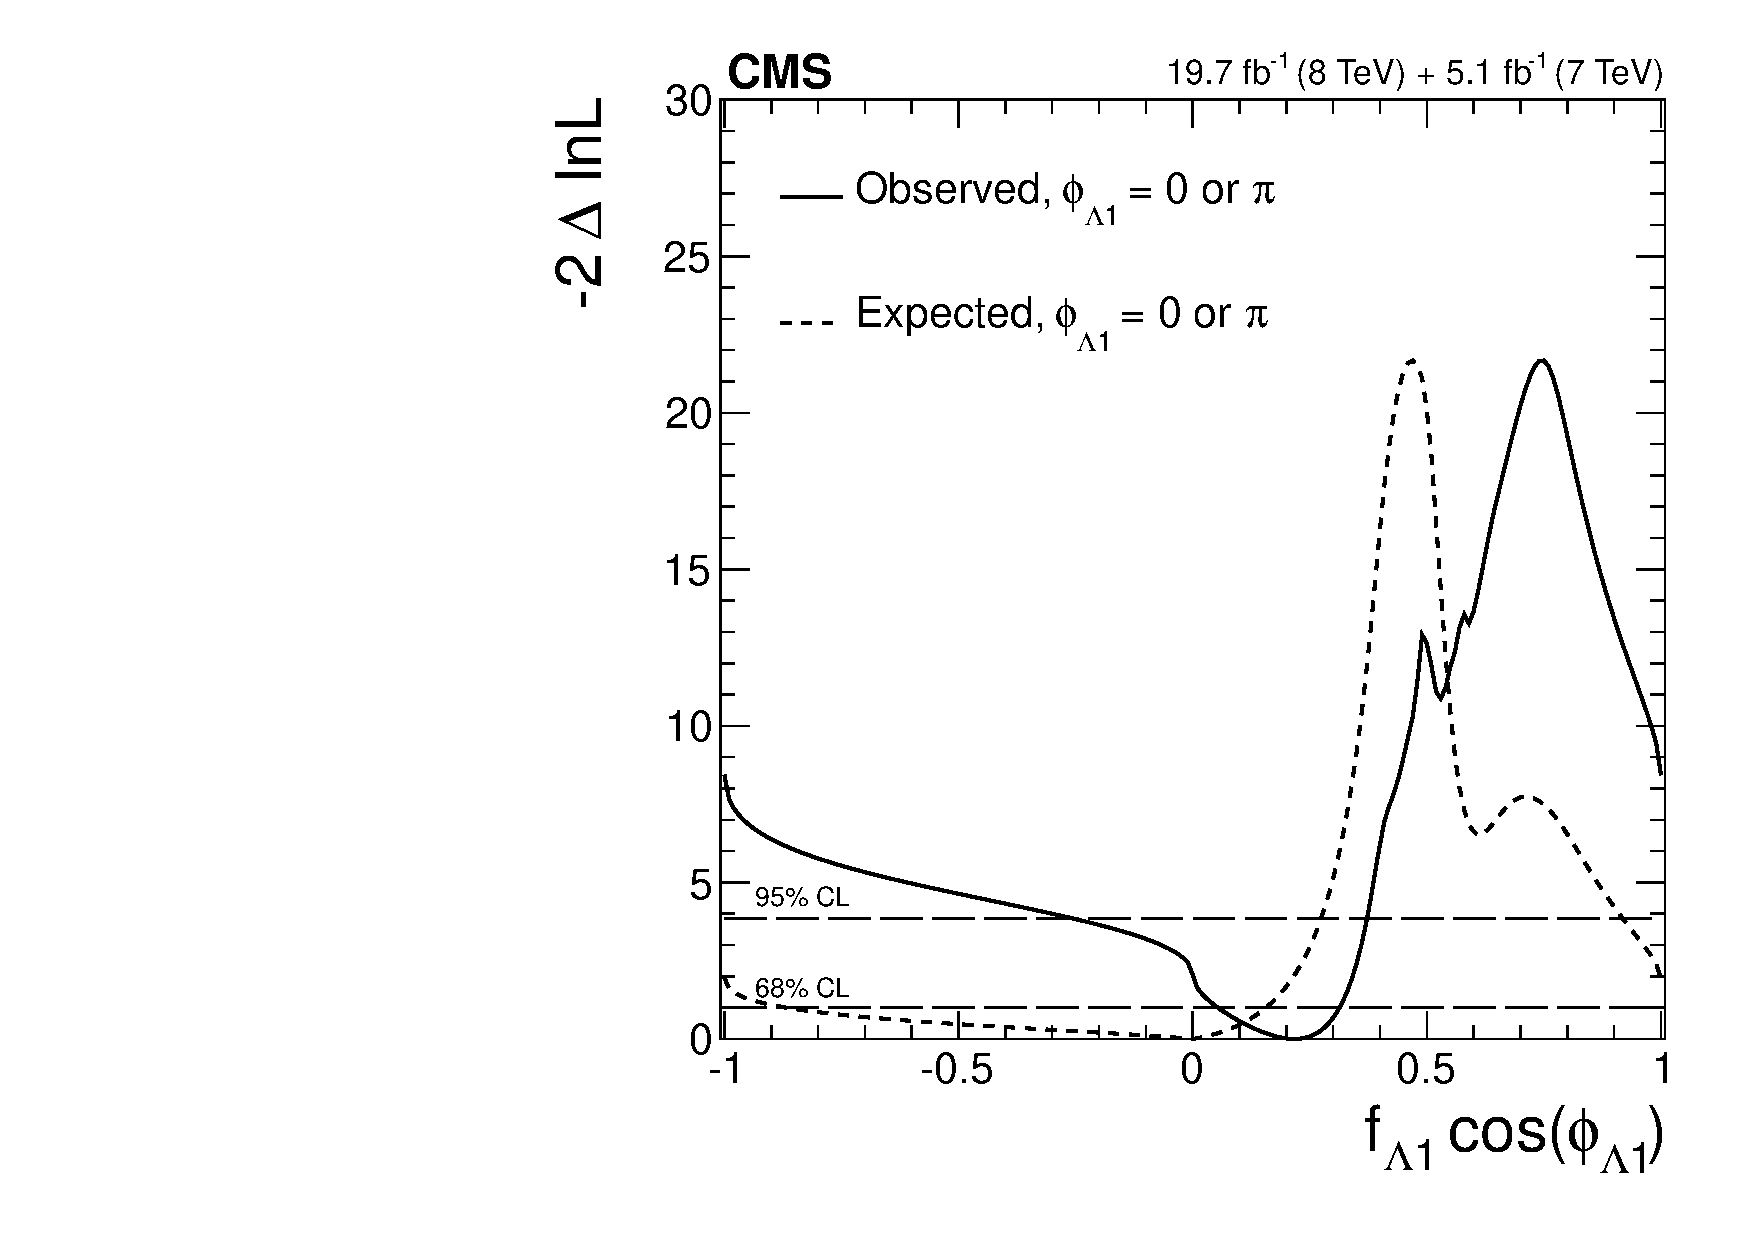
\includegraphics[width=0.31\linewidth,angle=0]{figures/fL1_Real.pdf}
%%        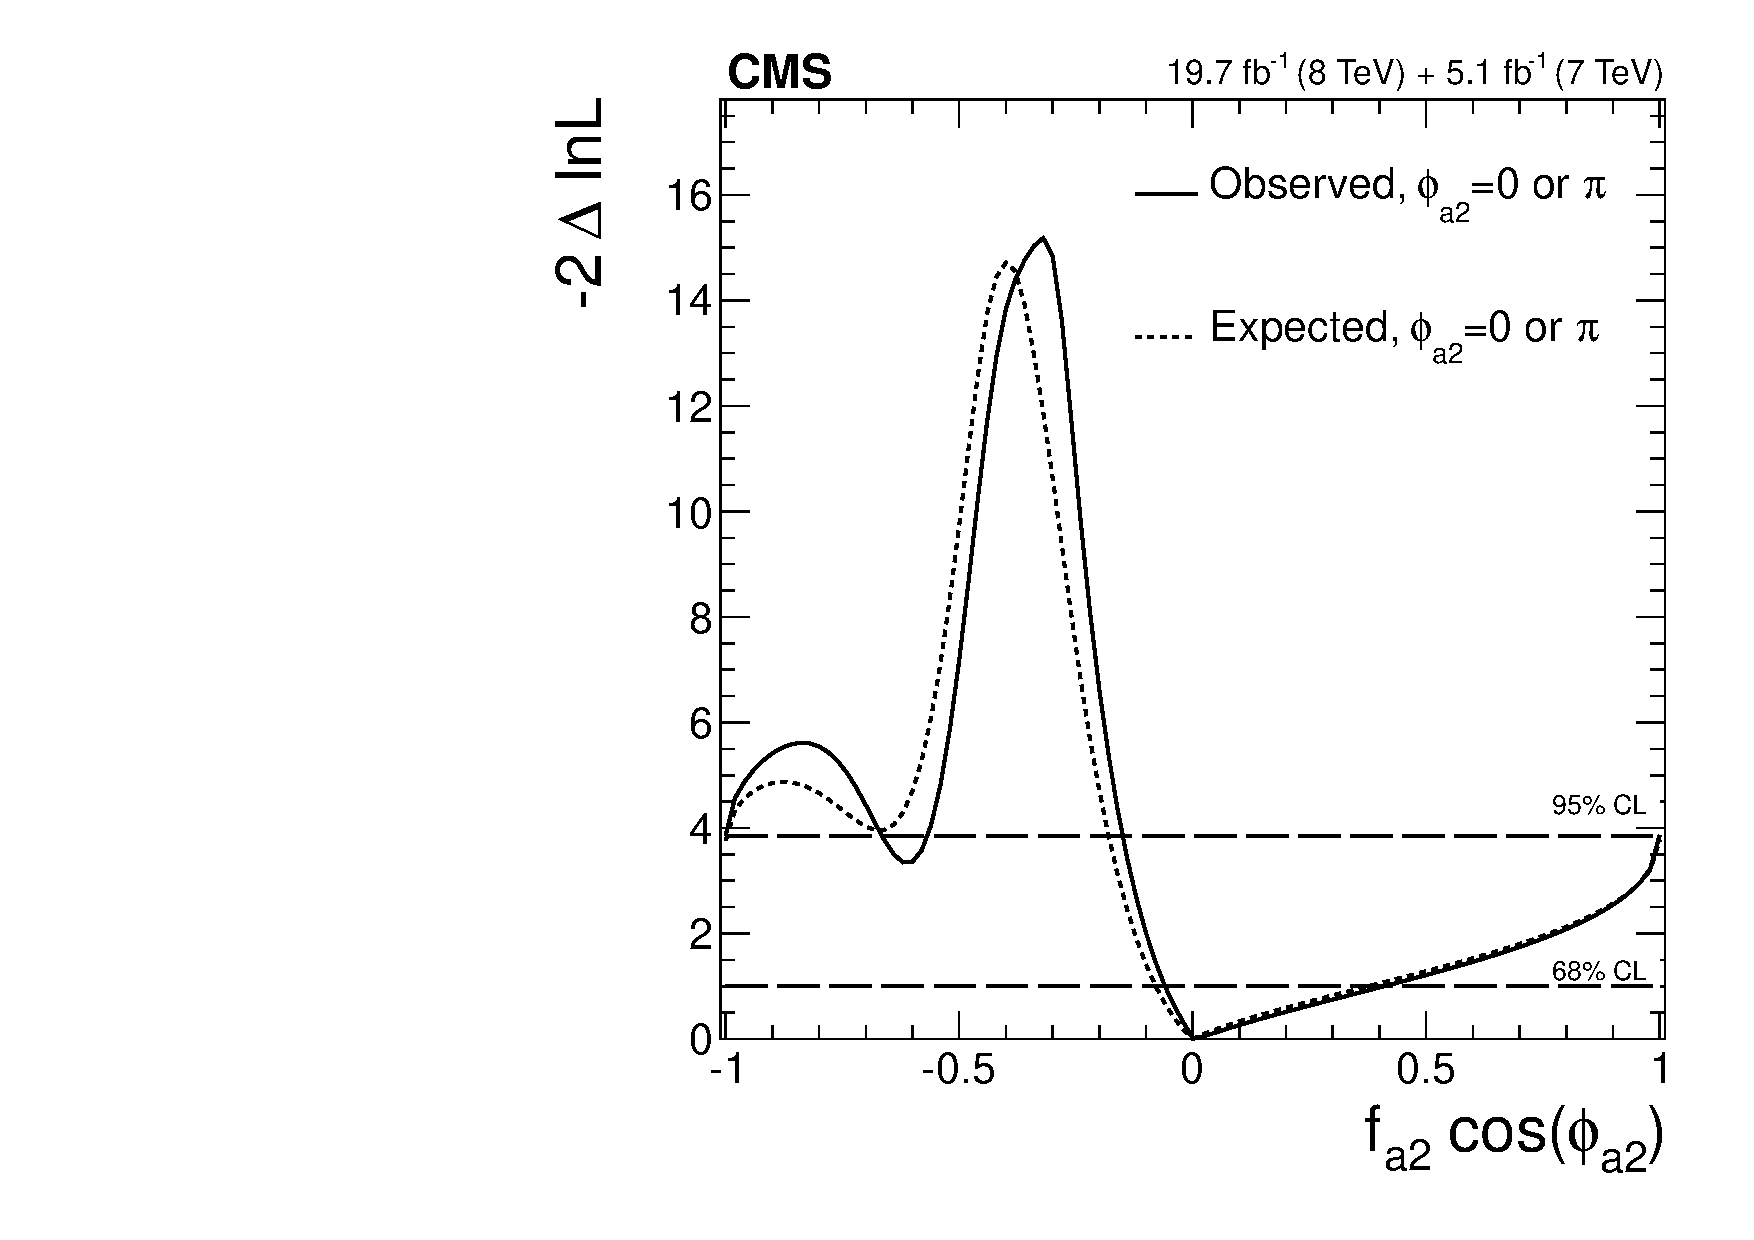
\includegraphics[width=0.31\linewidth,angle=0]{figures/fa2_Real.pdf}
%%        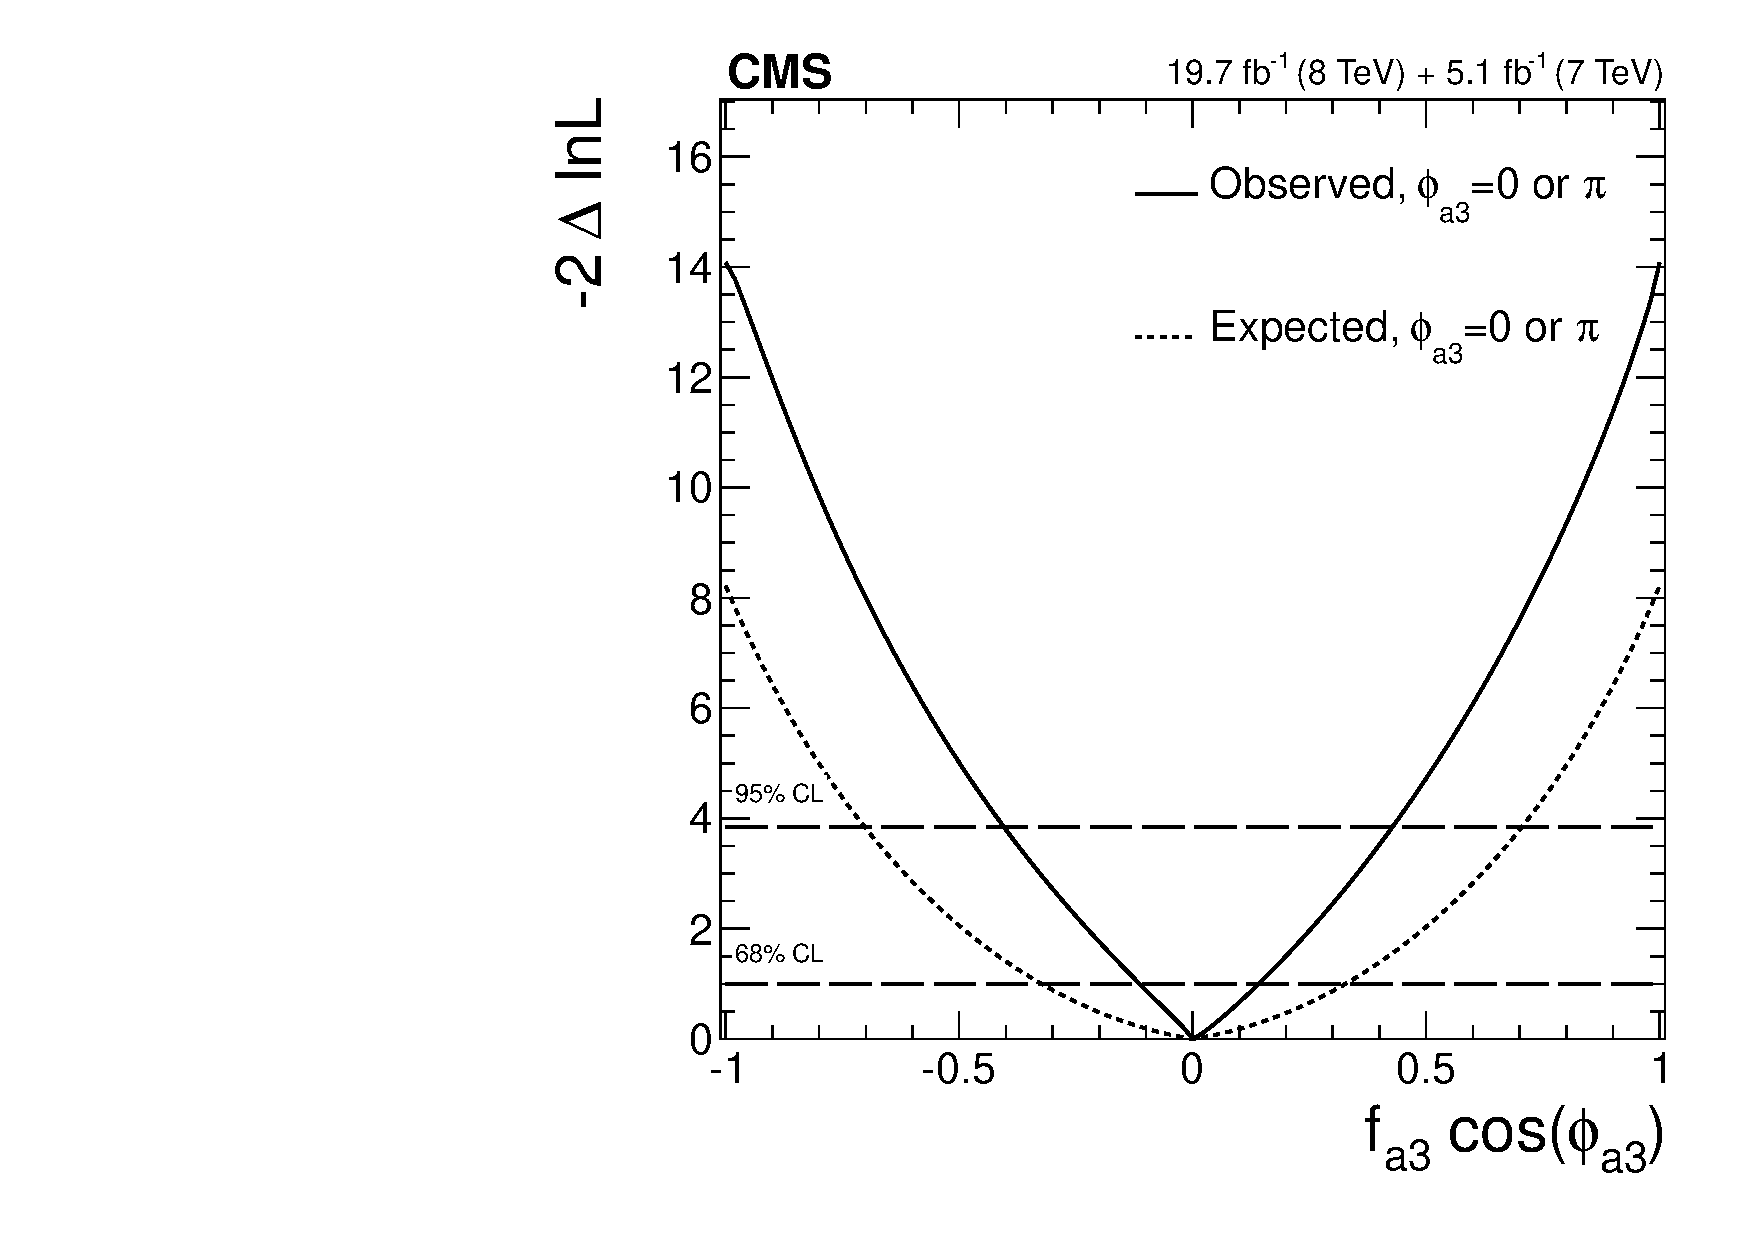
\includegraphics[width=0.31\linewidth,angle=0]{figures/fa3_Real.pdf}
%%         \caption{
%%         Expected (dashed) and observed (solid) likelihood scans using the template method for 
%%         the effective fractions $f_{\Lambda1}$, $f_{a2}$, $f_{a3}$ (from left to right) describing $\PH\PZ\PZ$ interactions. 
%%         The plots show the results when the couplings studied are constrained to be real and all other couplings are fixed to the SM predictions. 
%%         The $\cos\phi_{ai}$ term allows a signed quantity where $\cos\phi_{ai}=-1$ or $+1$.
%%         \label{fig:results_ZZ_1D}
%%         }
%% \end{center}
%% \end{figure}
%%%%%%%%%%%%%%%%%%%%%%%%%


  \item Simultaneous measurement of more than one-anomalous coupling.
    The same conclusions are reached by fitting one parameter and
    leaving another one to be unconstrained, in the full allowed
    parameter space, with $0\le f_{ai}\le 1$, in the hypothesis of
    real couplings. This tests the possible simultaneous
    presence of more than one anomalous contribution to the amplitude
    of Eq.~(\ref{eq:formfact-fullampl-spin0}). Results are consistent
    with SM-only amplitude: the two-dimensional scans of the
    likelihood in the case of real phases are shown in
    Fig.~\ref{fig:results_ZZ_2D} (top). All other parameters are
    constrained to be the SM ones. The measurements of $f_{a2}$ and $f_{a3}$ are also
    performed with the 8-dimensional likelihood, yielding to a consistent result.
\item The same simultaneous measurements can be performed in the case
  of generic phases, resulting in weaker constraints, but with fewer
  assumptions. Likelihood scans for three pairs of couplings with
  generic phases are shown in Fig.~\ref{fig:results_ZZ_2D} (bottom).

%%%%%%%%%%%%%%%%%%%%%%%%%
\begin{figure}[!p]
\begin{center}
        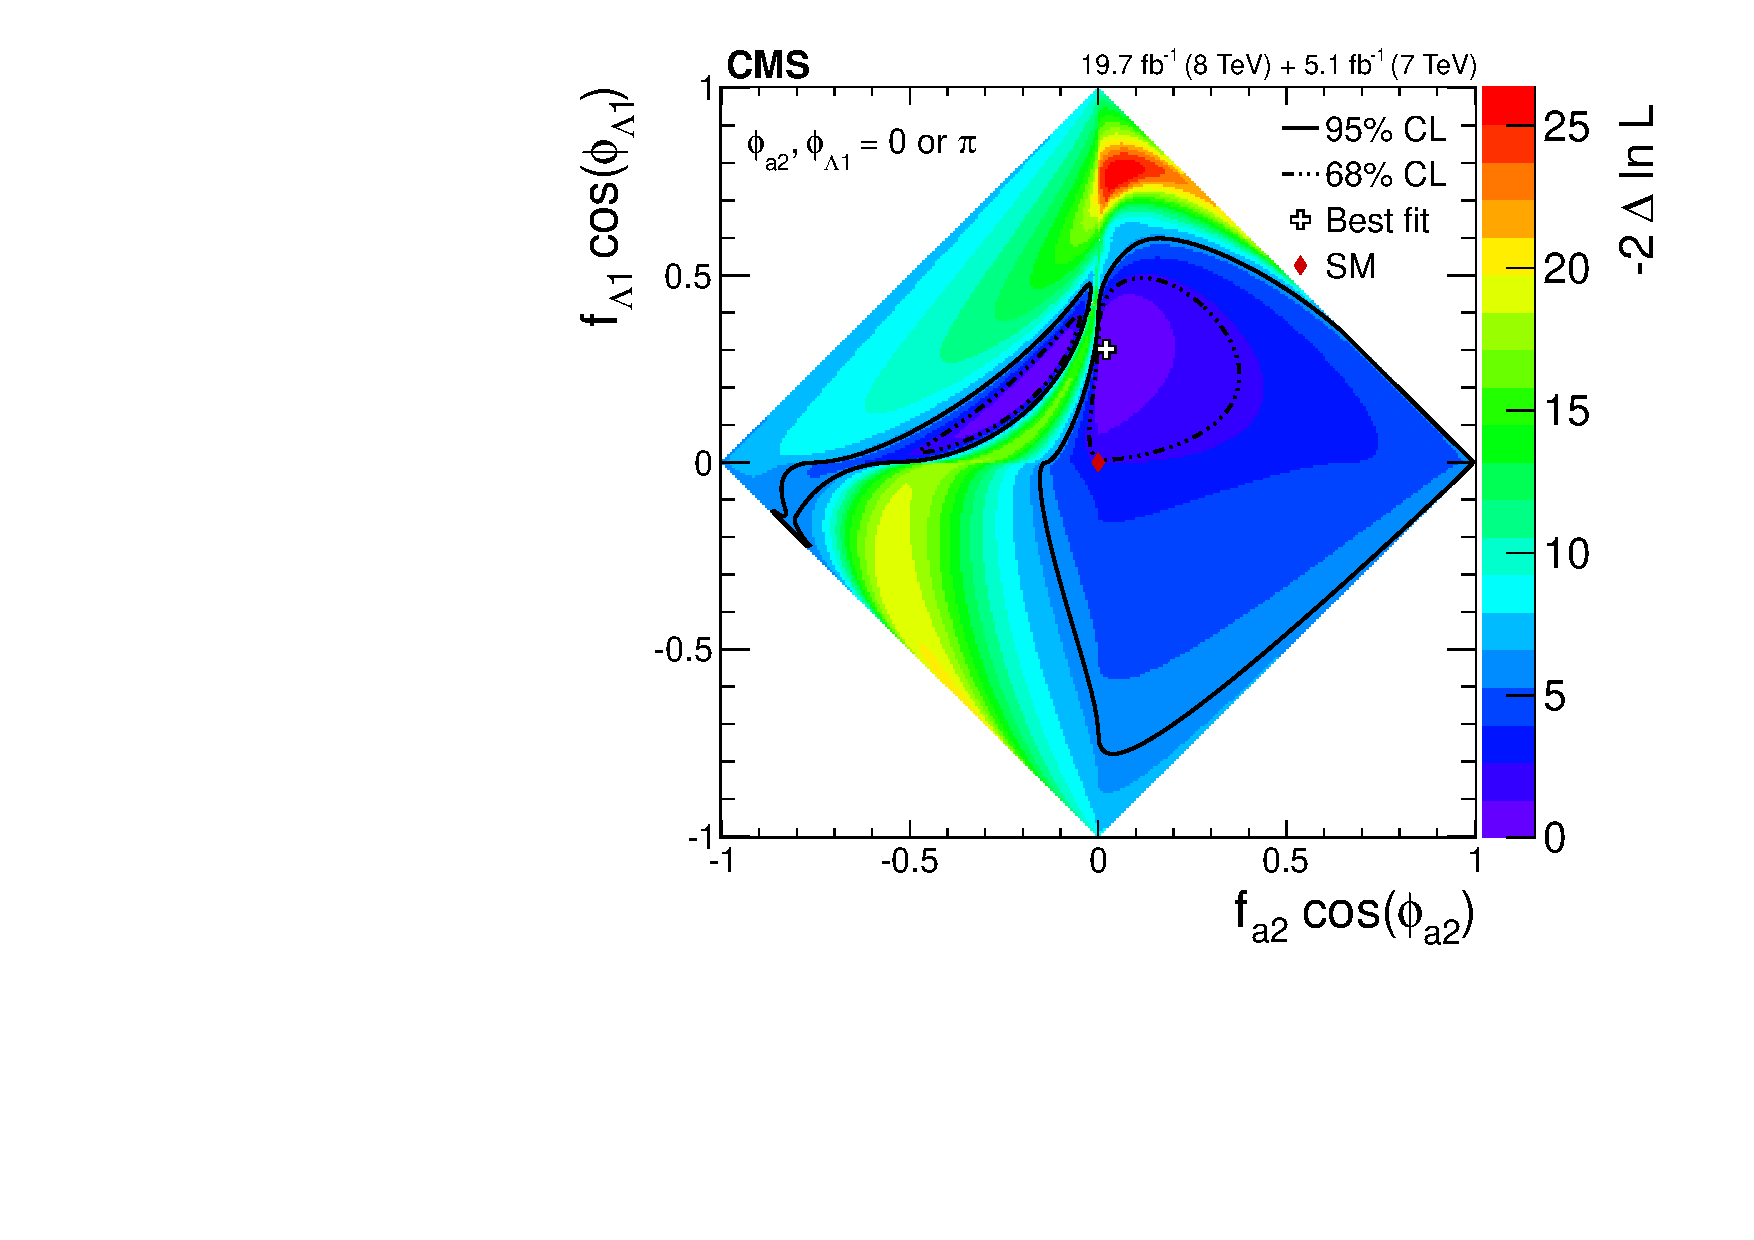
\includegraphics[width=0.31\linewidth,angle=0]{figures/fL1_vs_fa2_Real.pdf}
        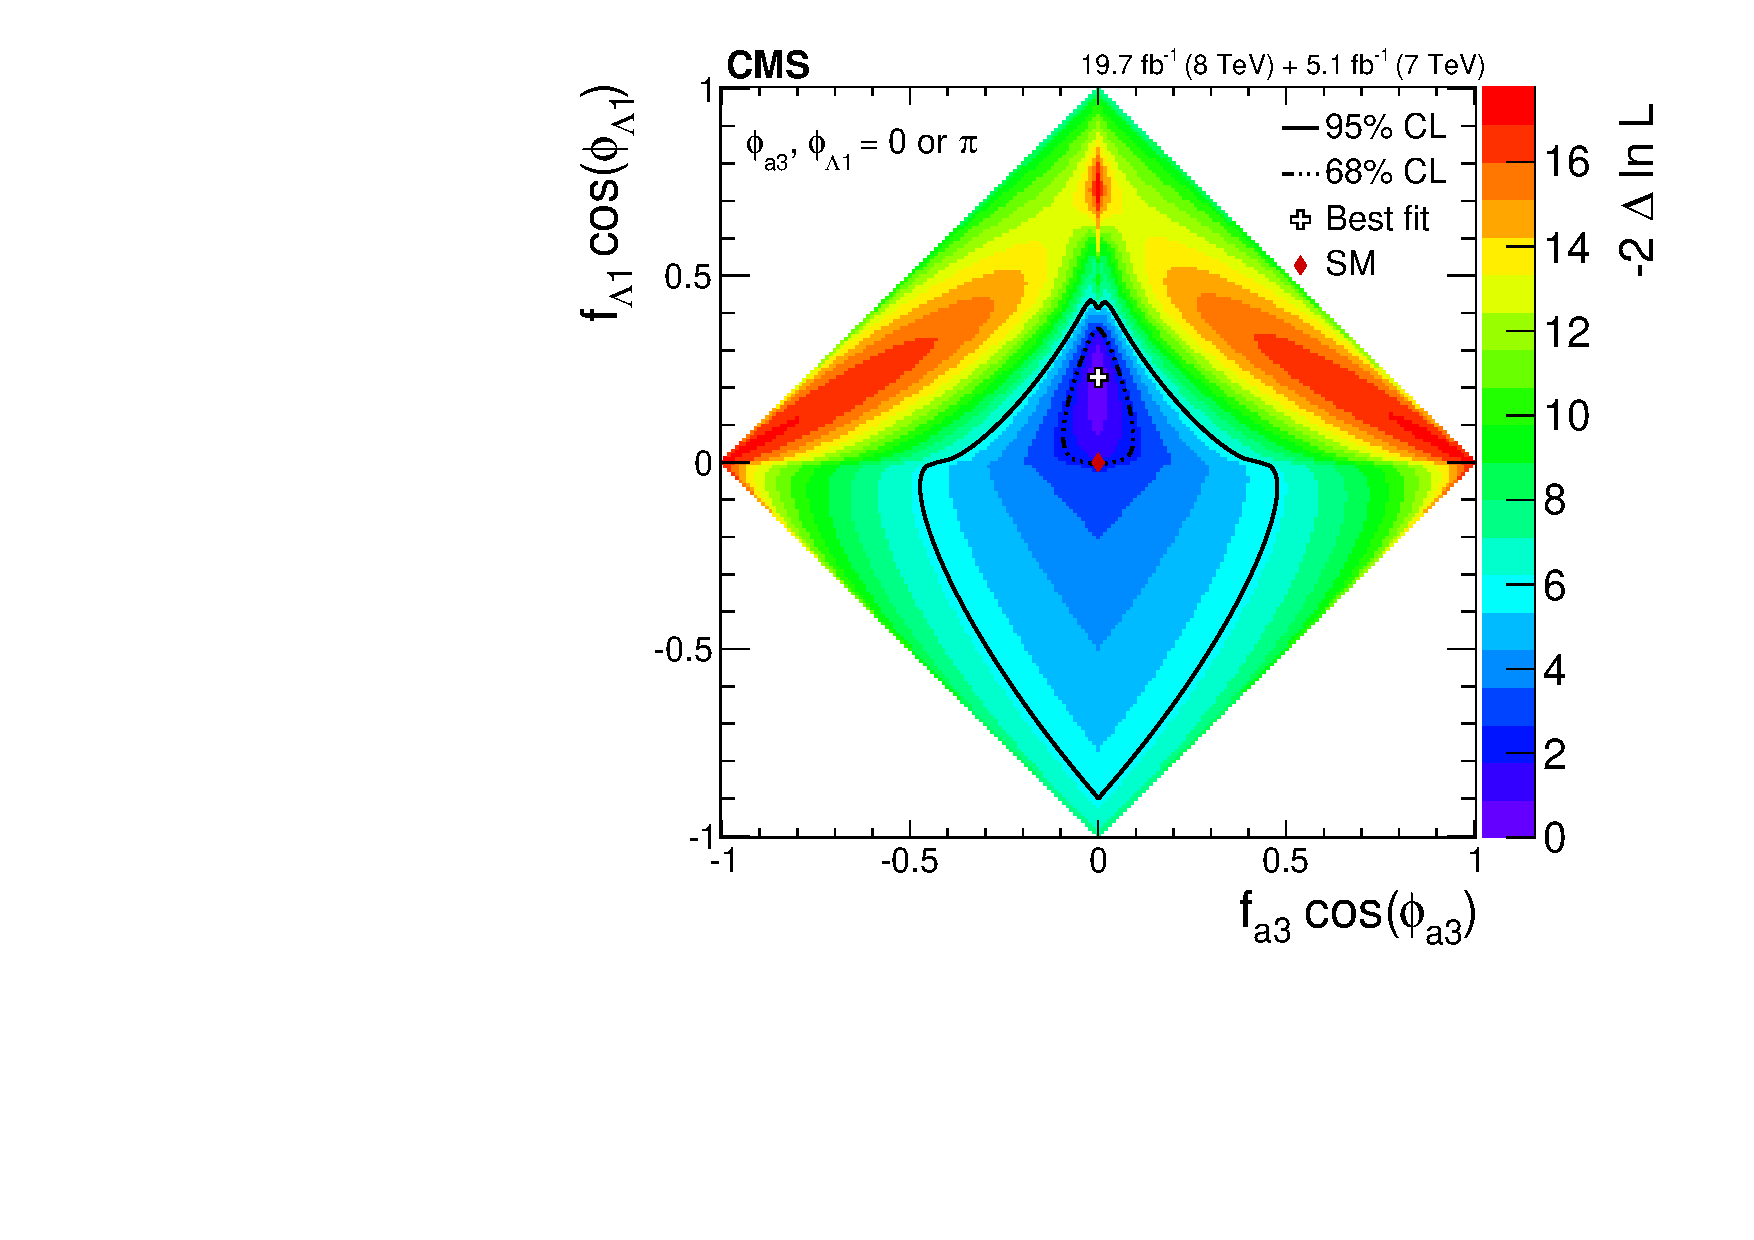
\includegraphics[width=0.31\linewidth,angle=0]{figures/fL1_vs_fa3_Real.pdf}
        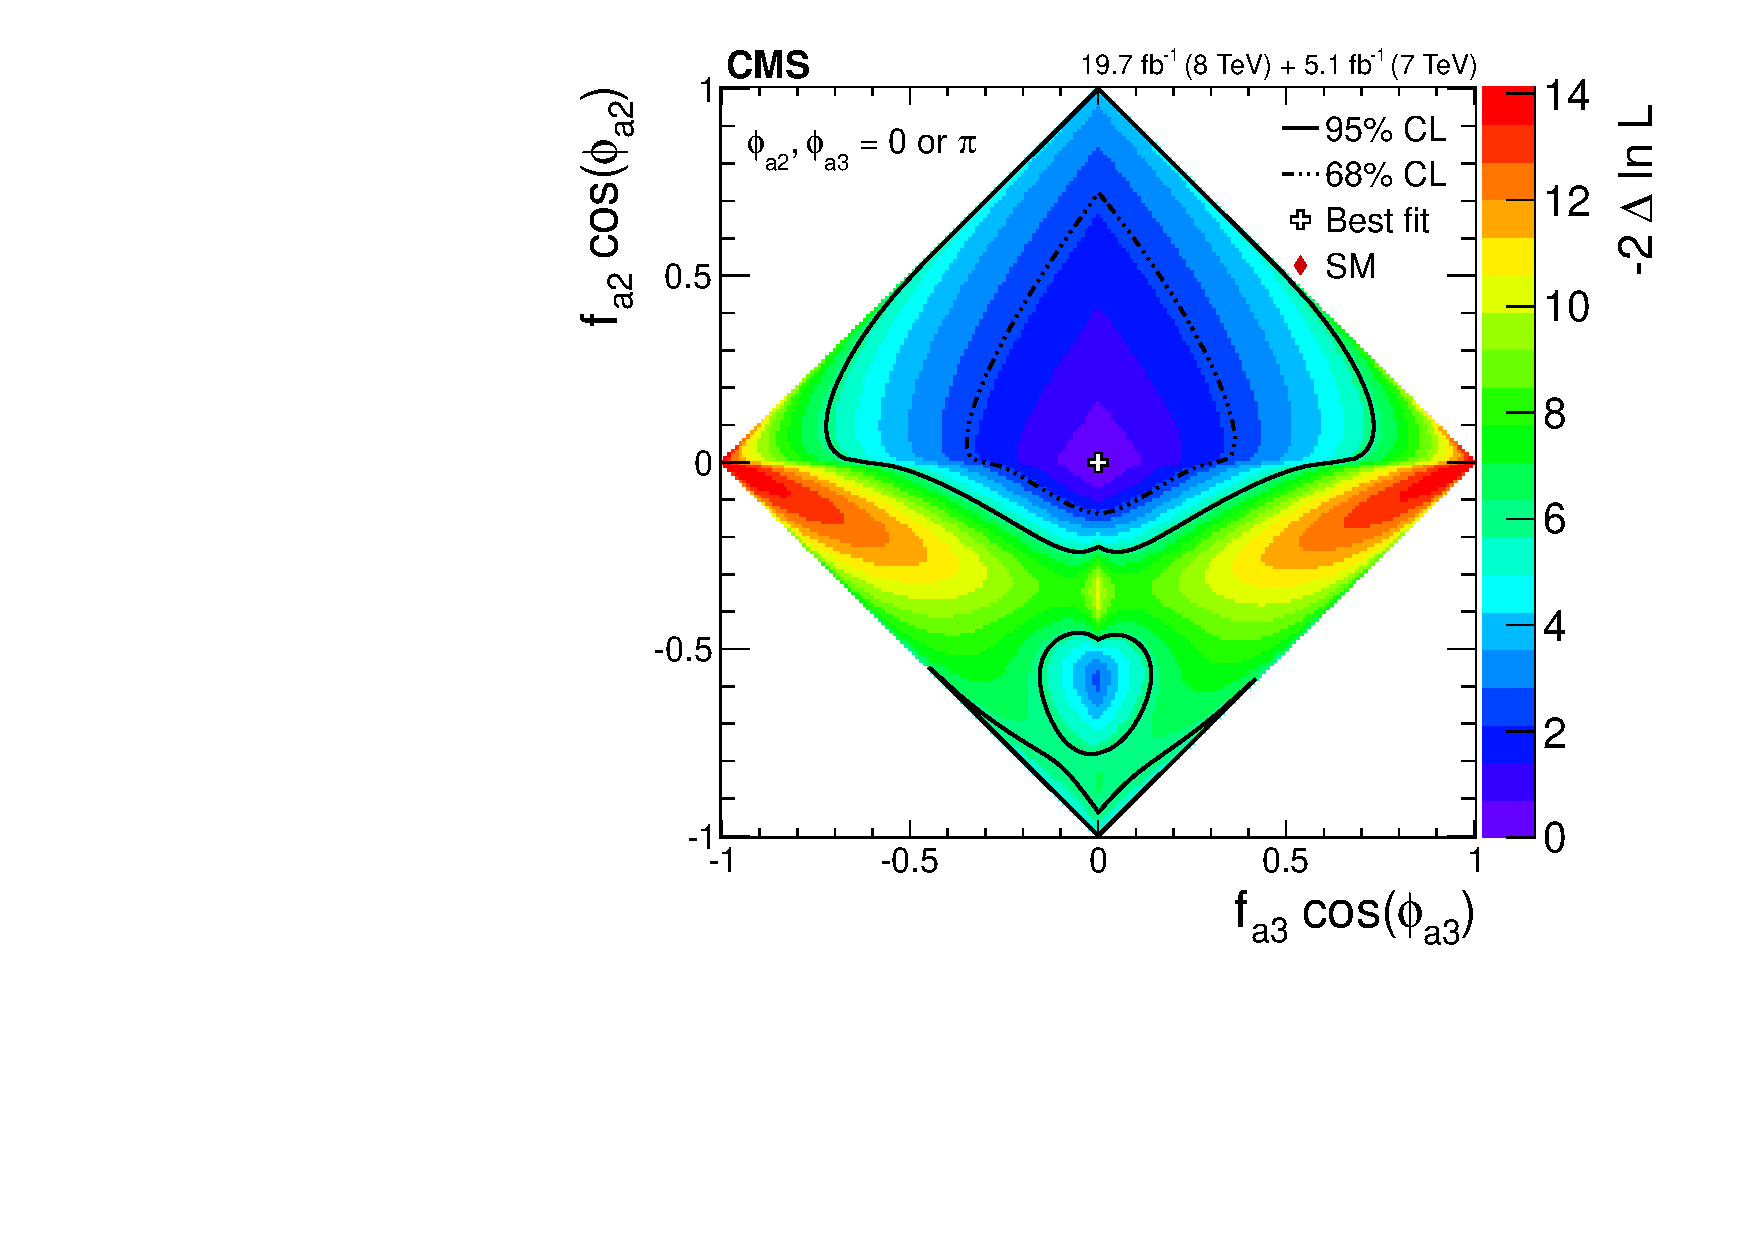
\includegraphics[width=0.31\linewidth,angle=0]{figures/fa2_vs_fa3_Real.pdf} \\
        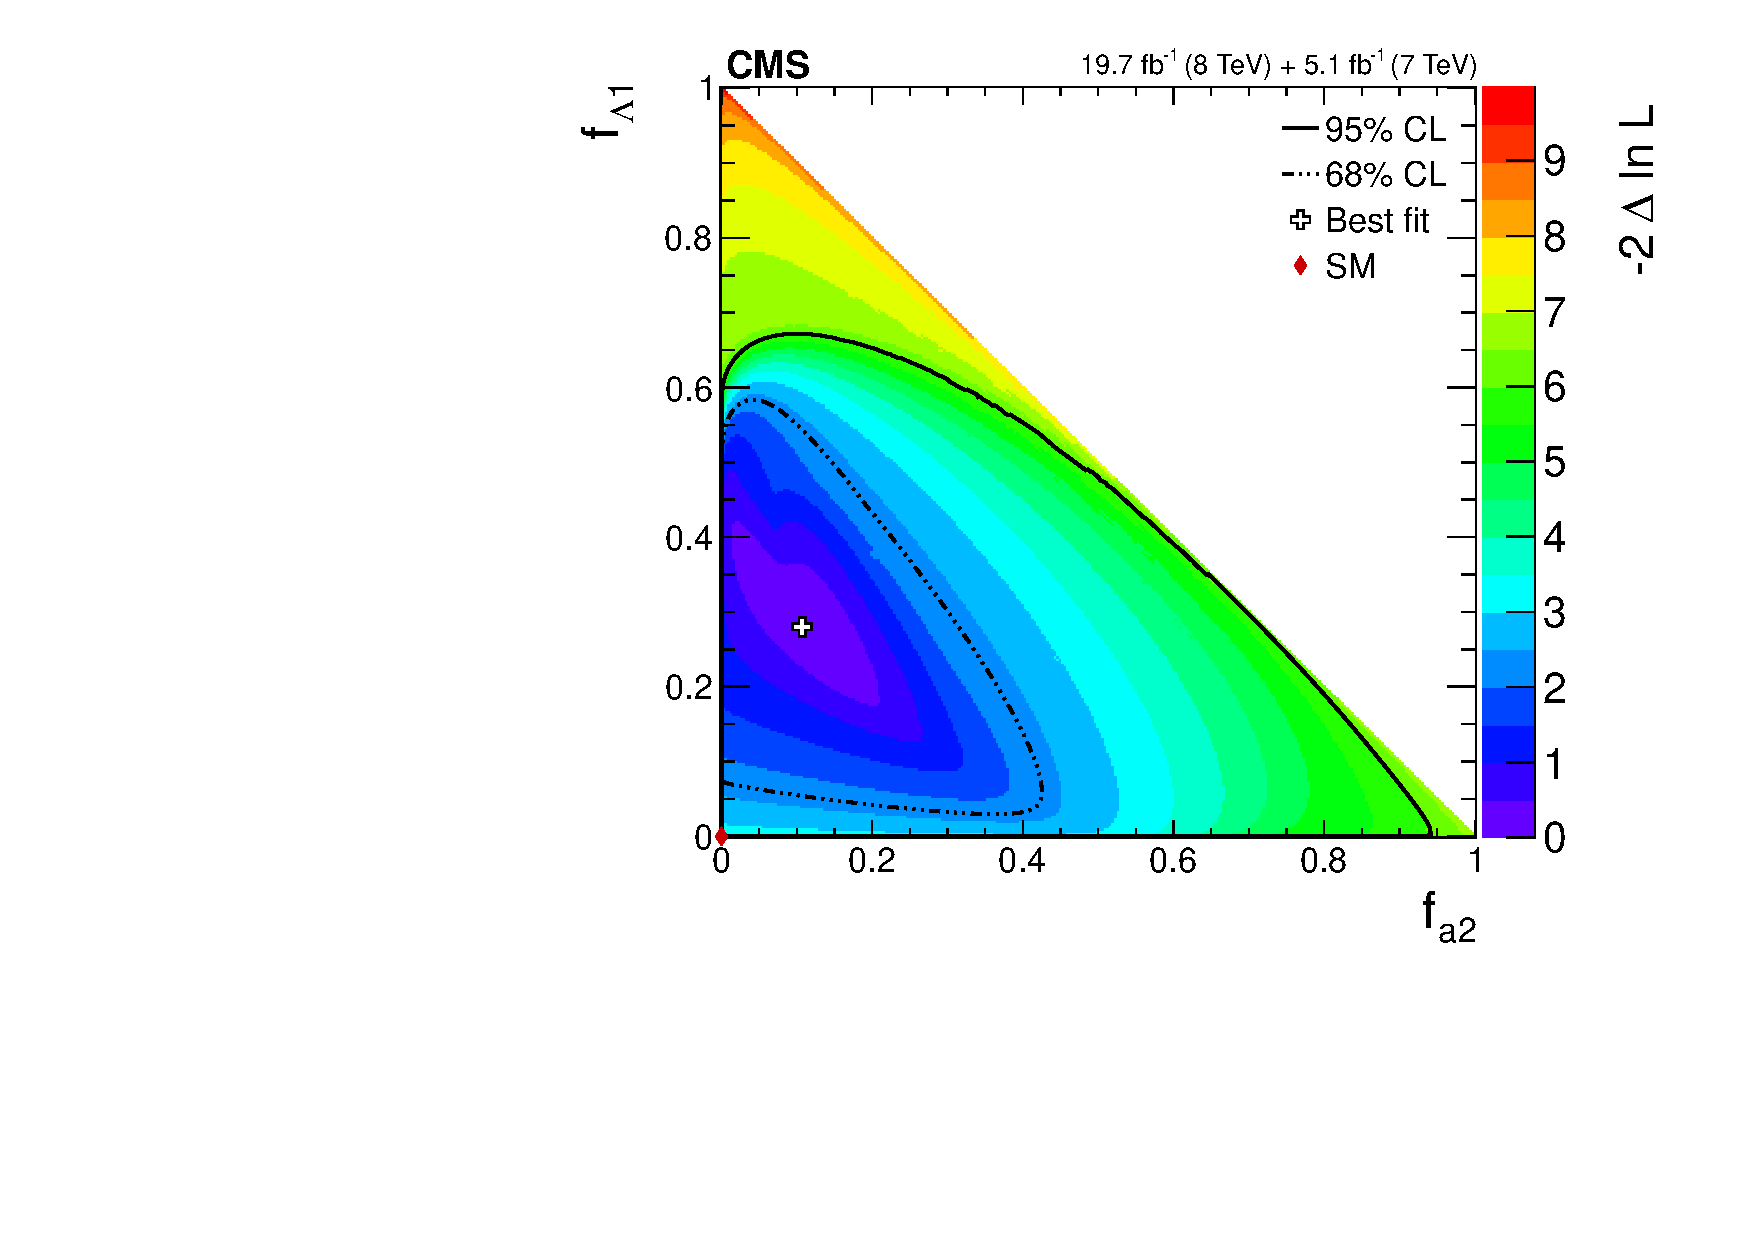
\includegraphics[width=0.31\linewidth,angle=0]{figures/fL1_vs_fa2_Profile.pdf}
        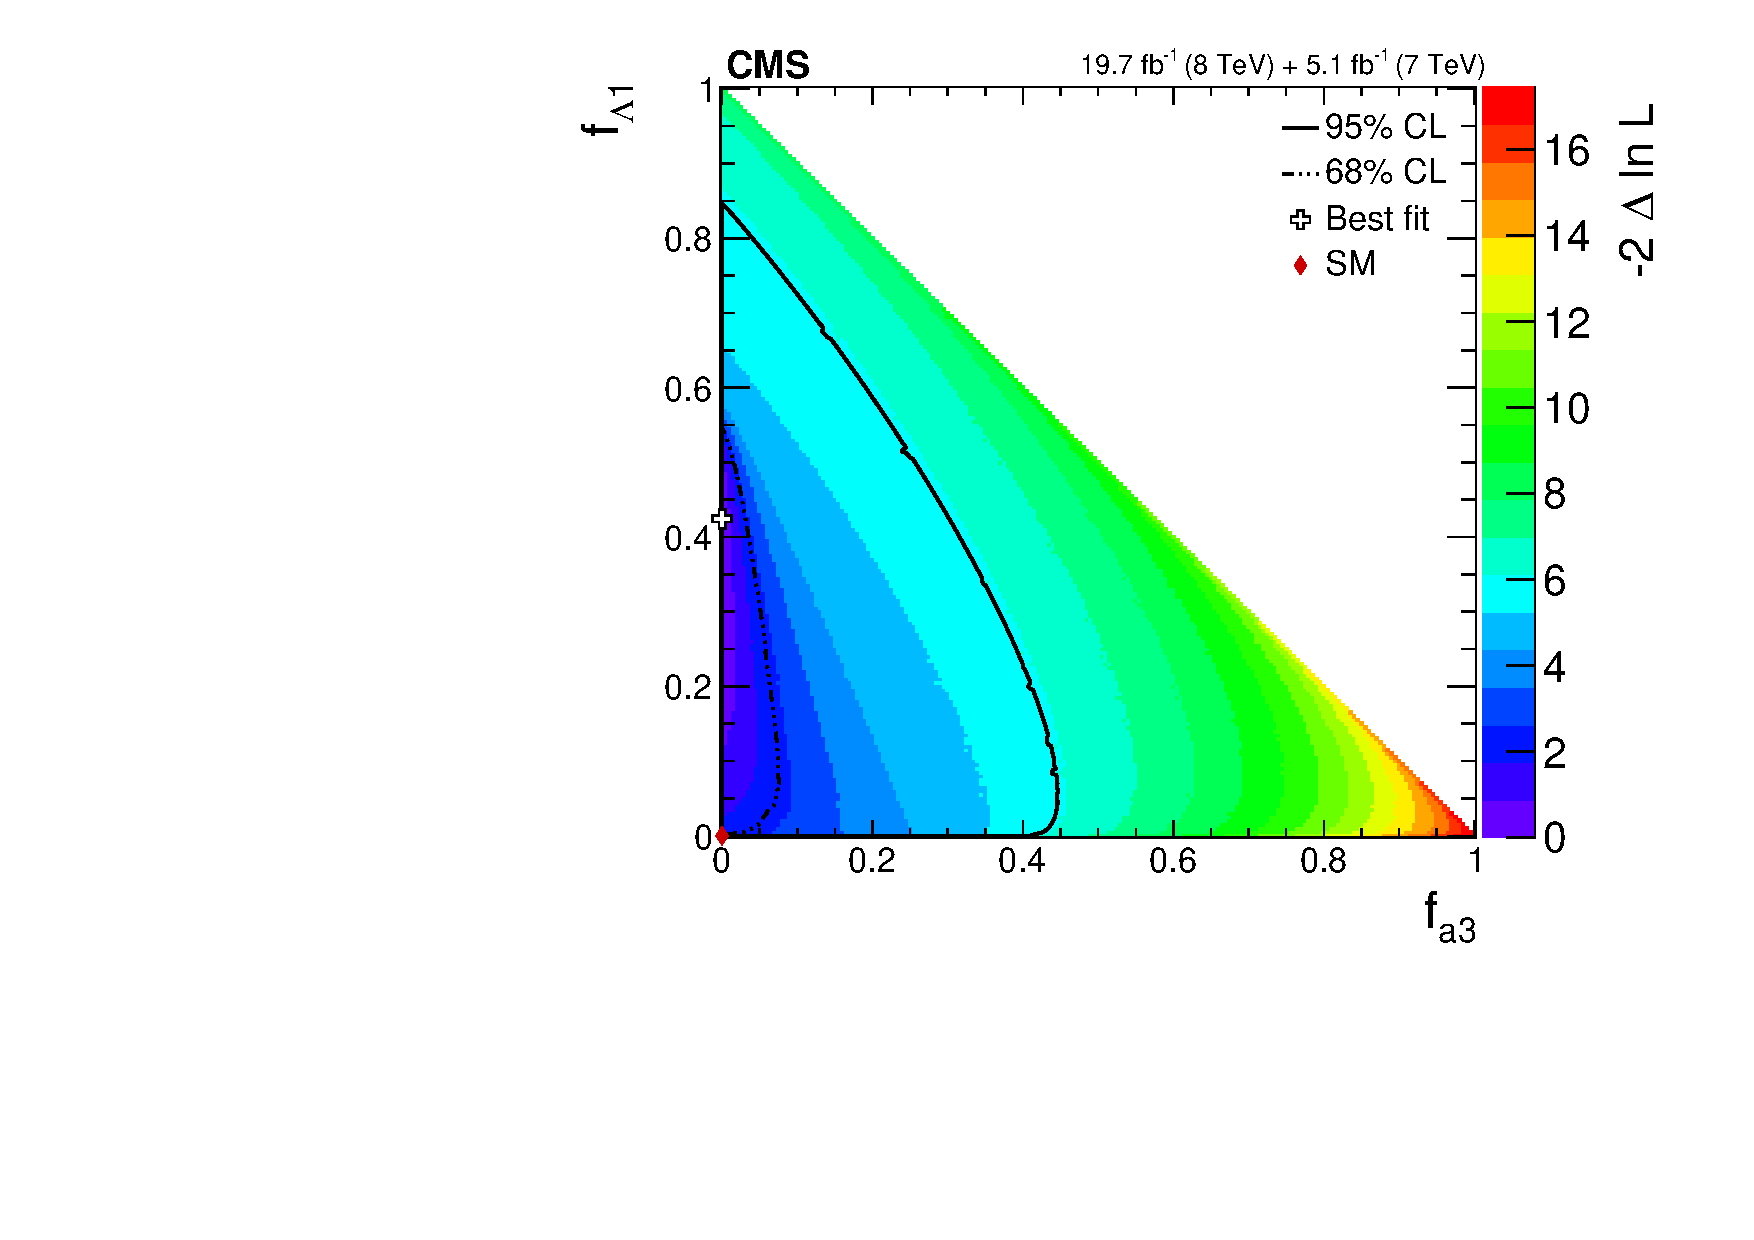
\includegraphics[width=0.31\linewidth,angle=0]{figures/fL1_vs_fa3_Profile.pdf}
        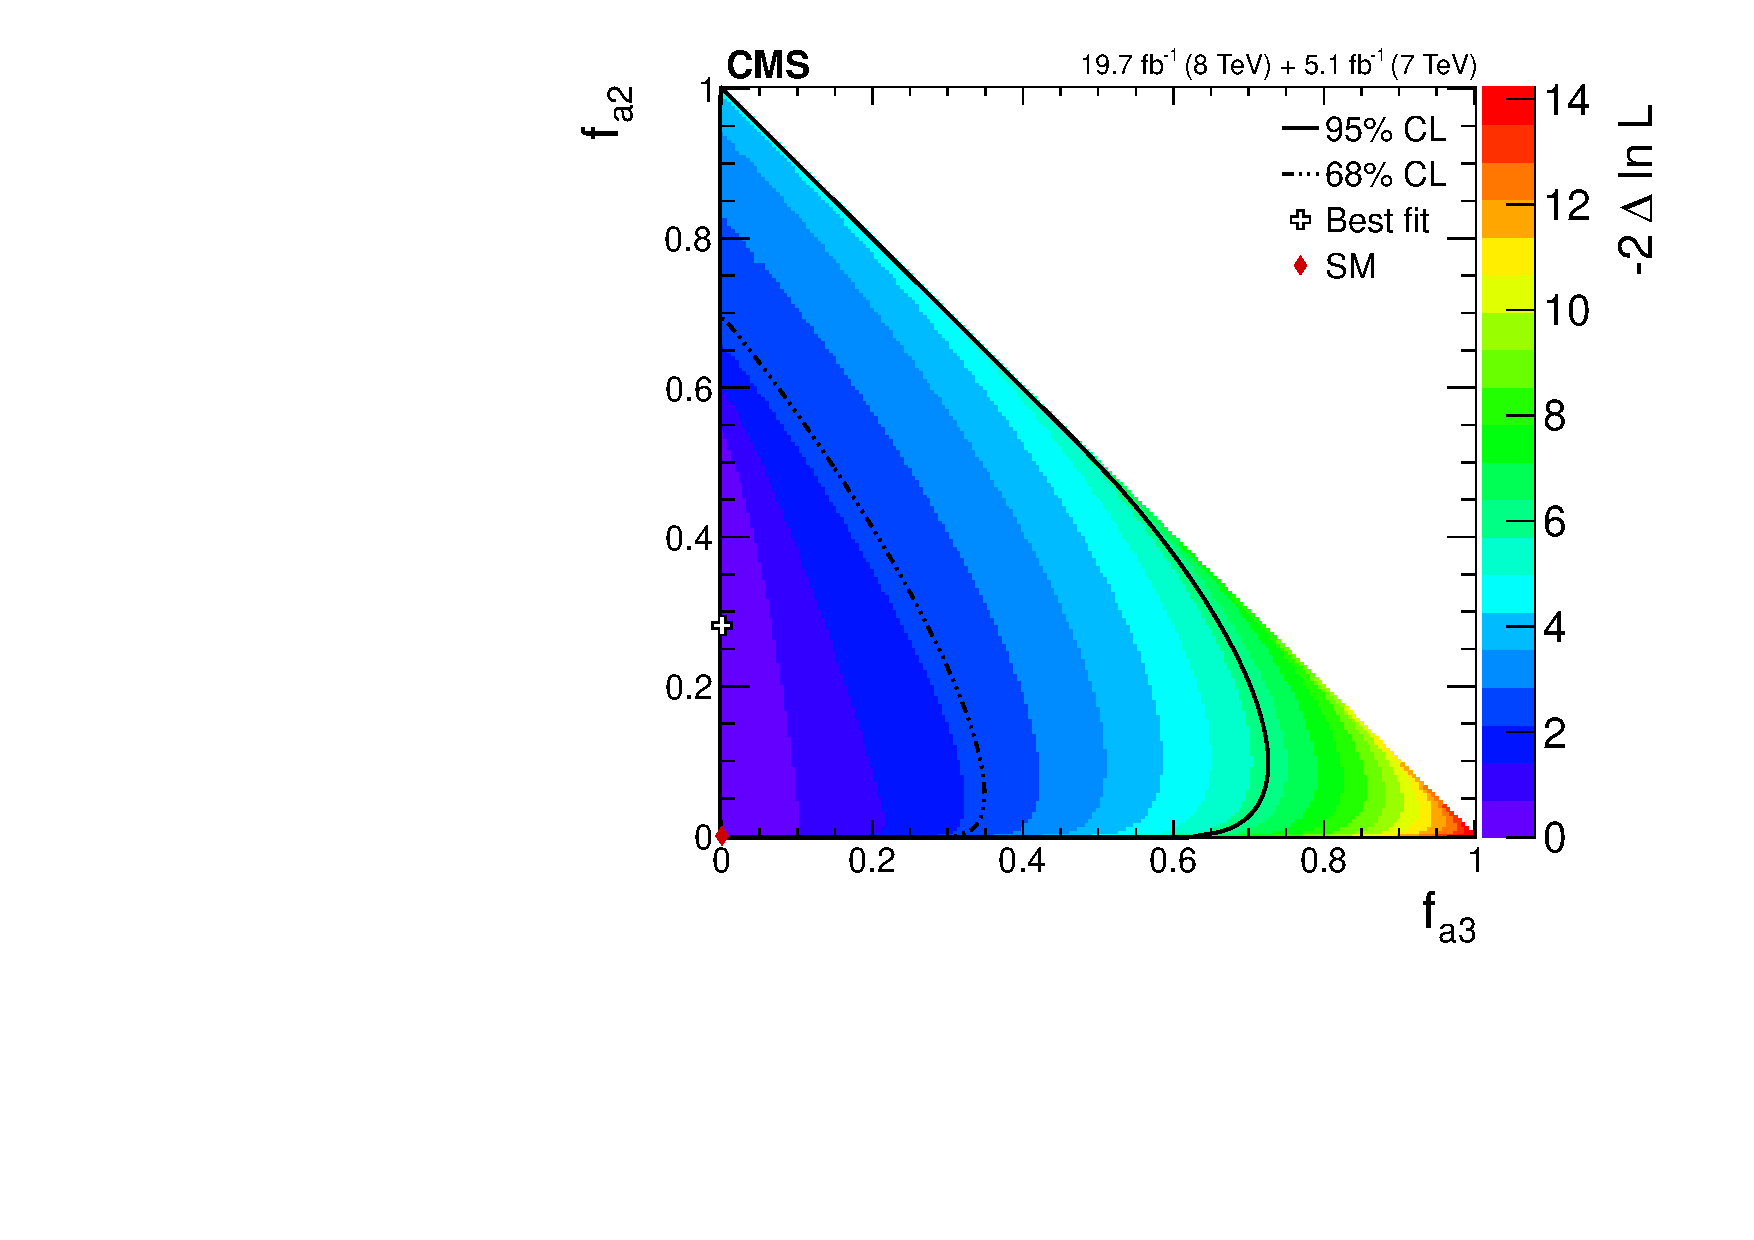
\includegraphics[width=0.31\linewidth,angle=0]{figures/fa2_vs_fa3_Profile.pdf}
        \caption{
        Observed likelihood scans using the template method for pairs of effective fractions $f_{\Lambda1}$ vs. $f_{a2}$, 
        $f_{\Lambda1}$ vs. $f_{a3}$, and $f_{a2}$ vs. $f_{a3}$ (from top to bottom) describing $\PH\PZ\PZ$ interactions. 
        The left column shows the results where the studied couplings are constrained to be real
        and all other couplings are fixed to the SM predictions.
        The right column shows the results when the phases of the anomalous couplings are left unconstrained. 
        \label{fig:results_ZZ_2D}
        }
\end{center}
\end{figure}
%%%%%%%%%%%%%%%%%%%%%%%%%

\end{enumerate}

The same set of measurements, presented for the $\chanHZZ$, can be
performed in the $\chanHWW$, though with reduced sensitivity, due to
the fewer kinematic observables available, and finally combined
together. For the latter, only real couplings, $\phi_{ai}^{\PW\PW}=0$
or $\pi$, are considered. The combination can be performed in two
scenarios, assuming custodial symmetry ($a_1^{WW} = a_1$), or not
assuming any ratio between the two scenarios. In the first case, the
relationships between the yield of $\chanHZZ$ and $\chanHWW$ yields to
a stronger constraint ont the anomalous couplings.
The likelihood scan for a particular value of $R_{ai}=0.5$ $(r_{ai} = 1)$
is shown in Fig.~\ref{fig:hwwscans}, where the stronger constraint from 
the yield relationship between the two channels is visible. When the custodial
symmetry is assumed, an even stronger constraint arise, strongly disfavouring 
the hypothesis of $f_{a2}=\pm1$.
%

%%%%%%%%%%%%%%%%%%%%%%%
\begin{figure}[!p]
  \begin{center} 
    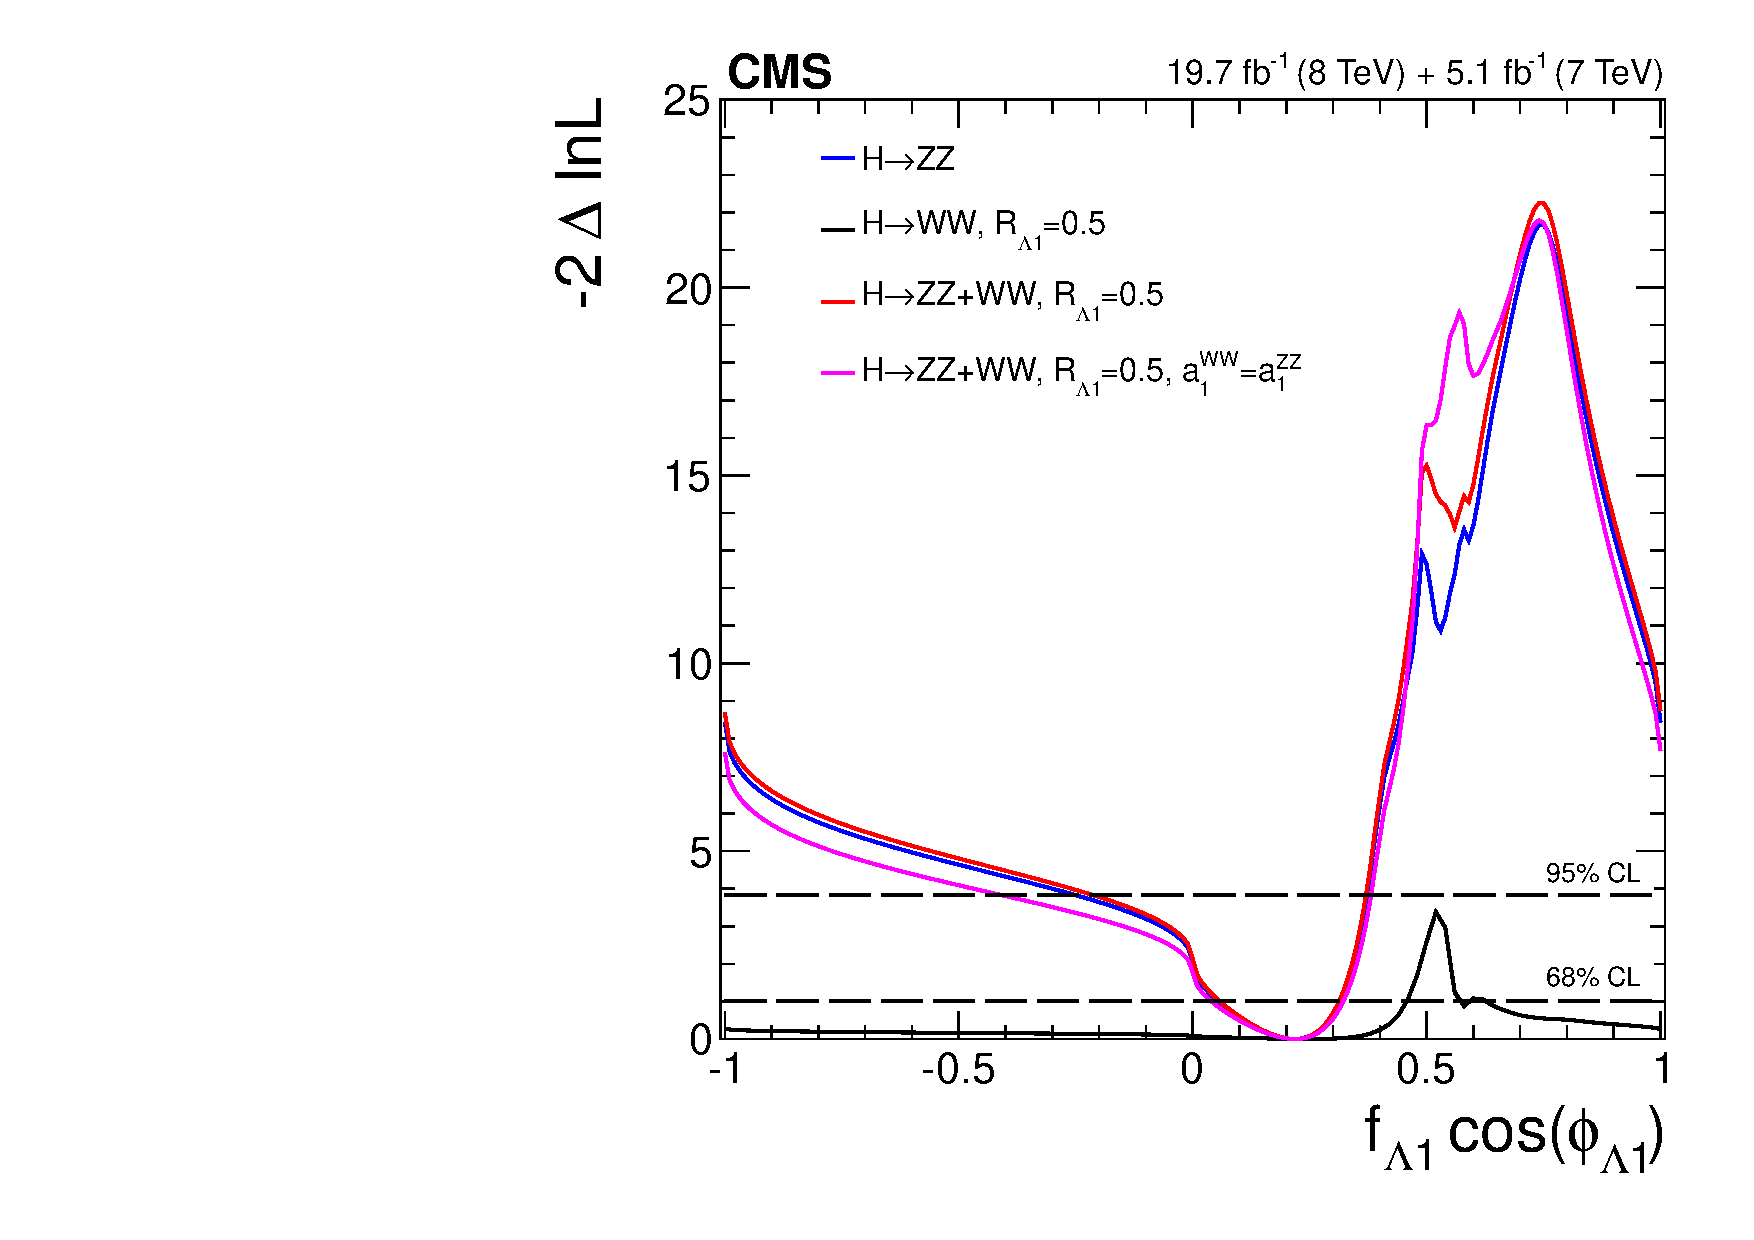
\includegraphics[width=0.31\linewidth]{figures/flambda1_combine_ww.pdf}
    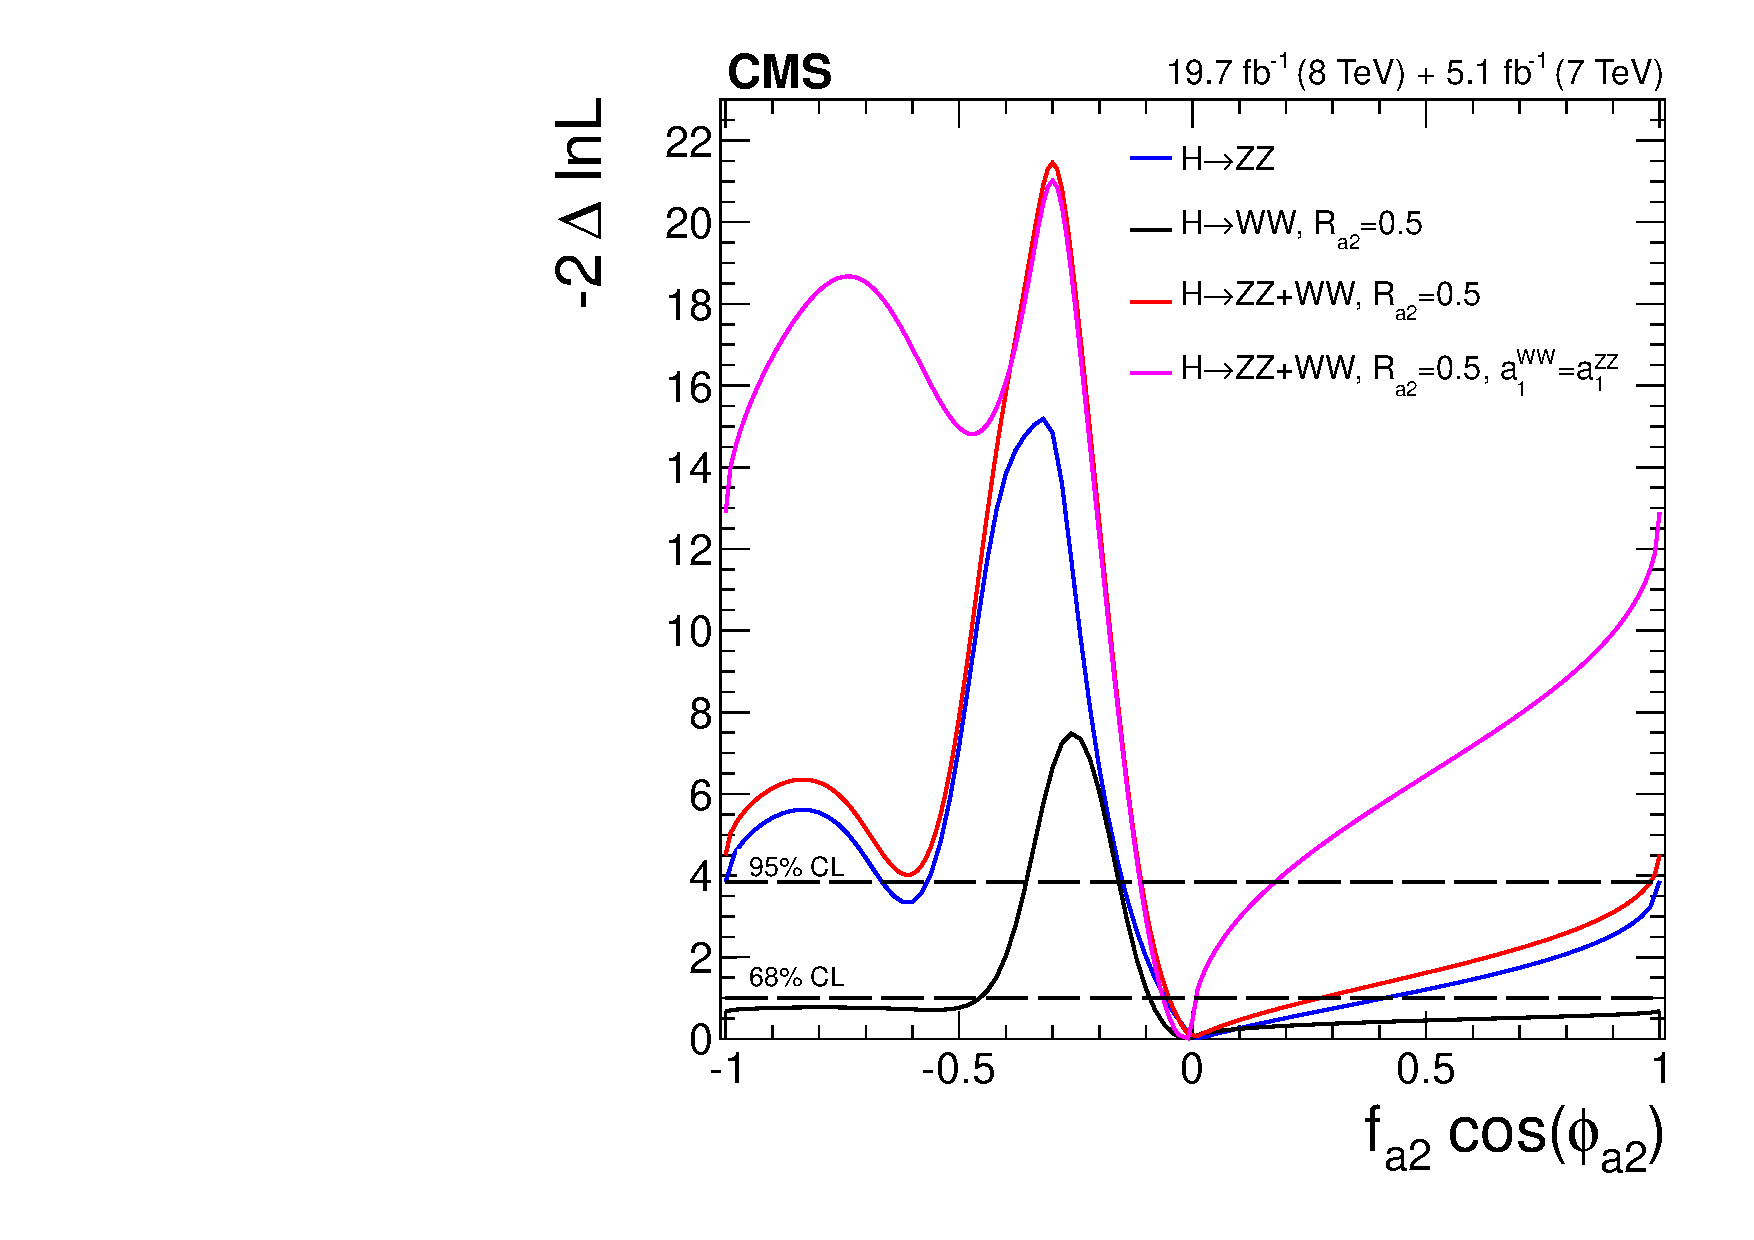
\includegraphics[width=0.31\linewidth]{figures/fa2_combine_ww.pdf}
    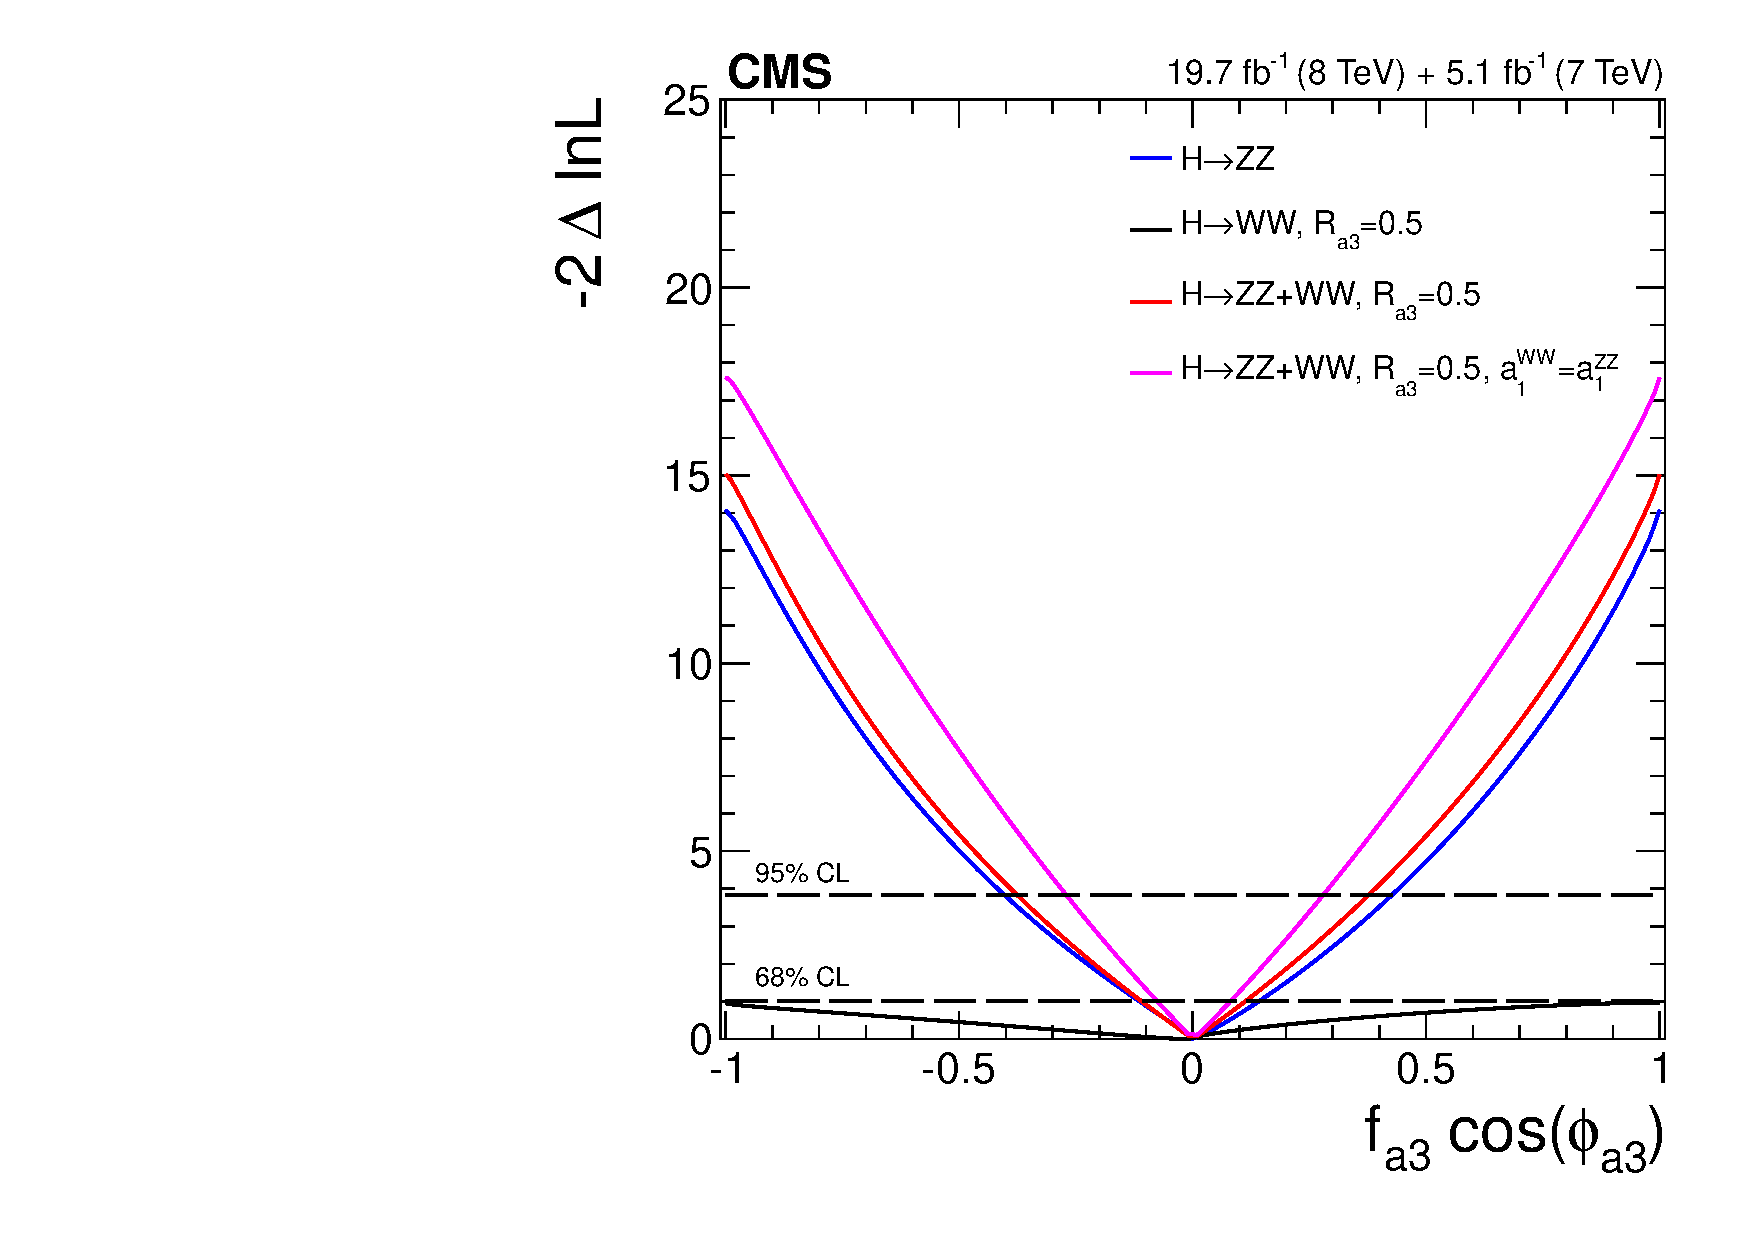
\includegraphics[width=0.31\linewidth]{figures/fa3_combine_ww.pdf}
    \caption{
      Expected and observed likelihood scans for effective fractions 
      $f_{\Lambda1}$ (left), $f_{a2}$ (middle), $f_{a3}$ (right). 
      The couplings studied are constrained to be real and all other anomalous couplings are fixed to the SM predictions. 
      The $\cos\phi_{ai}$ term allows a signed quantity where $\cos\phi_{ai}=-1$ or $+1$.
      The plots show the combined  $\PH\to\PW\PW$ and $\PH\to\PZ\PZ$ result in terms of the $\PH\PZ\PZ$ couplings for $R_{ai} = 0.5$. 
      Measurements are shown for each channel separately and two types of combination are present:
      using $a_1^{\PW\PW} = a_1$ (red) and without such a constraint (magenta).
    \label{fig:hwwscans}
    }
  \end{center}
\end{figure}
%%%%%%%%%%%%%%%%%%%%%%%

%
Overall, all anomalous $\PH\V\V$ couplings are found to be consistent
with zero, which is also consistent with the expectation from the SM
where these couplings are expected to be very small, well below the
current sensitivity.
